%% INTRO — Draft A: Spatial Generalization framing
\section{Introduction}
\label{sec:intro}

Vision-Language-Action (VLA) models have achieved remarkable in-distribution

\begin{figure*}[t]
\centering
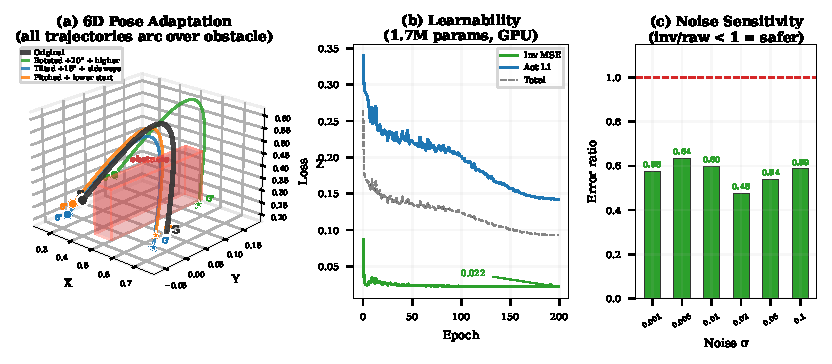
\includegraphics[width=0.95\textwidth]{teaser}
\vspace{-3mm}
\caption{\textbf{\dhb{} overview.}
\textbf{(a)} VLAs degrade 14--18\% under spatial shift; \dhb{} adapts in 7\,ms with 0\,mm error.
\textbf{(b)} 6D pose adaptation from a single demo --- different start orientations, shape preserved.
\textbf{(c)} Per-trial invariance: DHB MSE $\sim 10^{-33}$ vs raw $\sim 0.5$ (40 SE(3) transforms).}
\label{fig:teaser}
\end{figure*}
performance: StarVLA reaches 97.8\% on LIBERO~\cite{starvla_2026},
OpenVLA-OFT reaches 97.1\%~\cite{openvla_oft_2025}, and
ACoT-VLA reaches 98.5\%~\cite{acot_vla_2026}.
Yet all of these models degrade sharply under spatial distribution shift:
OpenVLA-OFT falls to 79.6\% ($-17.5\%$), StarVLA to 79.7\% ($-18.1\%$),
and ACoT-VLA to 84.1\% ($-14.4\%$) when the workspace changes.

\textbf{We identify the root cause as coordinate-frame dependence.}
All current VLA action representations --- discrete bins, \fast{}-compressed
tokens~\cite{fast2025}, continuous regression heads --- are functions of
absolute world or camera coordinates.
When a table height changes by $10\,\text{cm}$, the token stream changes completely
and the policy fails.
This is not a capacity limitation --- it is a representational flaw.

\textbf{We propose \dhb{}, an invariant trajectory encoding framework
for VLA spatial generalization.}
\dhb{} encodes end-effector trajectories in the $\se{3}$-quotient space of
motion-shape modulo pose, producing tokens whose magnitude components are
\emph{provably invariant} to any rigid-body transform of the workspace.
DHB magnitude tokens change $0.0\%$ under random SE(3) transforms vs $99.1\%$ for raw action tokens.
At test time, a $\leq\!7\,\text{ms}$ geometric adaptation step re-grounds the
encoded trajectory to any new pose without retraining, re-encoding, or
additional demonstrations.

\textit{Encode once in invariant space; adapt geometrically at 7\,ms.}

\paragraph{Contributions.}
\begin{enumerate}
\item \textbf{Invariant spatial generalization.}
$0.0\,\text{mm}$ end-effector error at $10\,\text{cm}$ perturbation vs $100.0\,\text{mm}$
naive, in simulation with no retraining or additional demos.

\item \textbf{Geometry-aware tokenization.}
$0.0\%$ token change under SE(3) transforms vs $99.1\%$ for raw actions;
8 OAT-style tokens with prefix decodability ($k{=}1$: MSE $= 0.0013$).

\item \textbf{Sample efficiency.}
$N{=}1$ invariant-encoded demo covers any pose neighborhood;
equal spatial generalization to $N{=}20$ raw demos.

\item \textbf{Modular VLA integration.}
\texttt{DHBActionHeader} for StarVLA as a drop-in action head,
enabling controlled ablation of invariant vs non-invariant tokenization
on the same Qwen2.5-VL backbone.
\end{enumerate}
